% !TEX program = xelatex
\documentclass[11pt,a4paper]{ctexart}

\usepackage{amsmath,amssymb}
\usepackage{booktabs}
\usepackage{tabularx}
\usepackage{longtable}
\usepackage[margin=2.2cm]{geometry}
\usepackage{xcolor}
\usepackage{titlesec}
\usepackage{fancyhdr}
\usepackage{enumitem}
\usepackage{graphicx}
\usepackage{float}
\usepackage{caption}
\usepackage{hyperref}
\usepackage{array}
\usepackage{makecell}

\definecolor{deepblue}{RGB}{28,64,120}
\definecolor{warnred}{RGB}{160,30,30}
\definecolor{okgreen}{RGB}{20,110,60}
\definecolor{graylight}{RGB}{245,245,247}
\definecolor{rulegray}{RGB}{200,200,205}

\titleformat{\section}{\normalfont\Large\bfseries\color{deepblue}}{\thesection}{0.6em}{}
\titleformat{\subsection}{\normalfont\large\bfseries\color{deepblue}}{\thesubsection}{0.6em}{}
\titleformat{\subsubsection}{\normalfont\normalsize\bfseries}{\thesubsubsection}{0.6em}{}

\pagestyle{fancy}
\fancyhf{}
\fancyhead[L]{\small\color{deepblue}Cabinet-BNN 完整评测报告}
\fancyhead[R]{\small\thepage}
\renewcommand{\headrulewidth}{0.4pt}

\hypersetup{colorlinks=true,linkcolor=deepblue,urlcolor=deepblue,
            pdftitle={Cabinet-BNN 完整评测报告},bookmarksnumbered=true}

\setlist[itemize]{leftmargin=1.4em,topsep=2pt,itemsep=1.5pt,parsep=0pt}
\setlist[enumerate]{leftmargin=1.6em,topsep=2pt,itemsep=1.5pt,parsep=0pt}

\newcommand{\warn}[1]{\textcolor{warnred}{\textbf{#1}}}
\newcommand{\ok}[1]{\textcolor{okgreen}{\textbf{#1}}}

\newcommand{\keybox}[1]{%
  \begin{center}\begin{minipage}{0.95\textwidth}%
  \colorbox{graylight}{\begin{minipage}{0.93\textwidth}\vspace{3pt}#1\vspace{3pt}\end{minipage}}%
  \end{minipage}\end{center}}

\captionsetup{font=small,labelfont={bf,color=deepblue}}

\title{\vspace{-1.5cm}\textbf{\color{deepblue}Cabinet-BNN 完整评测报告}\\[4pt]
       \large HSH-64 码复现 · BNN 消融 · 热更改与遗忘量\\[2pt]
       \normalsize \textcolor{gray}{v1 · 2026-02-12}}
\author{}
\date{}

\begin{document}
\maketitle
\thispagestyle{fancy}

\begin{center}
\begin{minipage}{0.93\textwidth}
\small
\textbf{原则}：所有数字均来自本机实跑，脚本与产物路径可复现。\warn{负面结果照实报告。}\\
\textbf{环境}：Python 3.11.9 ｜ PyTorch 2.5.1+cu121 ｜ Rust 1.96 ｜ RTX 4060 Laptop 8\,GB
\end{minipage}
\end{center}

\vspace{0.3cm}
\tableofcontents
\newpage

% =====================================================================
\section{执行摘要}

\subsection{三句话结论}

\begin{enumerate}
\item \textbf{HSH-64 码可以精确复现} —— Recall@10 $= 0.7426$，距离几何与论文图 2 吻合；
      \textbf{桶结构分析证实容量从不是瓶颈}（v1 设计文档的「容量危机」判断是错的）。
\item \textbf{纯 LM 质量上，per-token 权重码不占优} —— 等参数预算下劣于全局共享权重。
      这是一个必须承认的负面结果。
\item \textbf{但在设计真正瞄准的目标上，它显著胜出} —— 每域独立码表的「热插拔」方案达到
      \ok{遗忘量 0.0000、可逆性精确恢复、本域精度 0.3278 超过联合训练上界 0.3264}。
\end{enumerate}

\subsection{关键数字总表}

\begin{center}
\begin{tabularx}{\textwidth}{@{}clXl@{}}
\toprule
\textbf{实验} & \textbf{指标} & \textbf{结果} & \textbf{参照} \\
\midrule
一 & Recall@10（后处理后） & \textbf{0.7426} & 论文 h512 = 0.7404 \\
一 & 正/负样本对距离 & 9.17 / 26.08 bit & 论文图 2 $\approx$ 8 / $\approx$ 28 \\
一 & 分离度 & \textbf{16.91 bit} & 论文 $\approx$ 18 \\
一 & 最大语义桶 & \textbf{3}（上限 256） & 准完美哈希可行 \\
二 & code vs shared（等参数） & 4.162 vs \textbf{3.973} & \warn{code 劣} \\
二 & code vs token\_embed & \textbf{4.162} vs 4.783 & \ok{code 优} \\
三 & code\_swap 遗忘量 & \textbf{0.0000} & shared\_ft = 0.0301 \\
三 & code\_swap 可逆性 & \textbf{精确恢复} & 其它方法均不精确 \\
\bottomrule
\end{tabularx}
\end{center}

% =====================================================================
\section{完整架构图}

\begin{figure}[H]
\centering
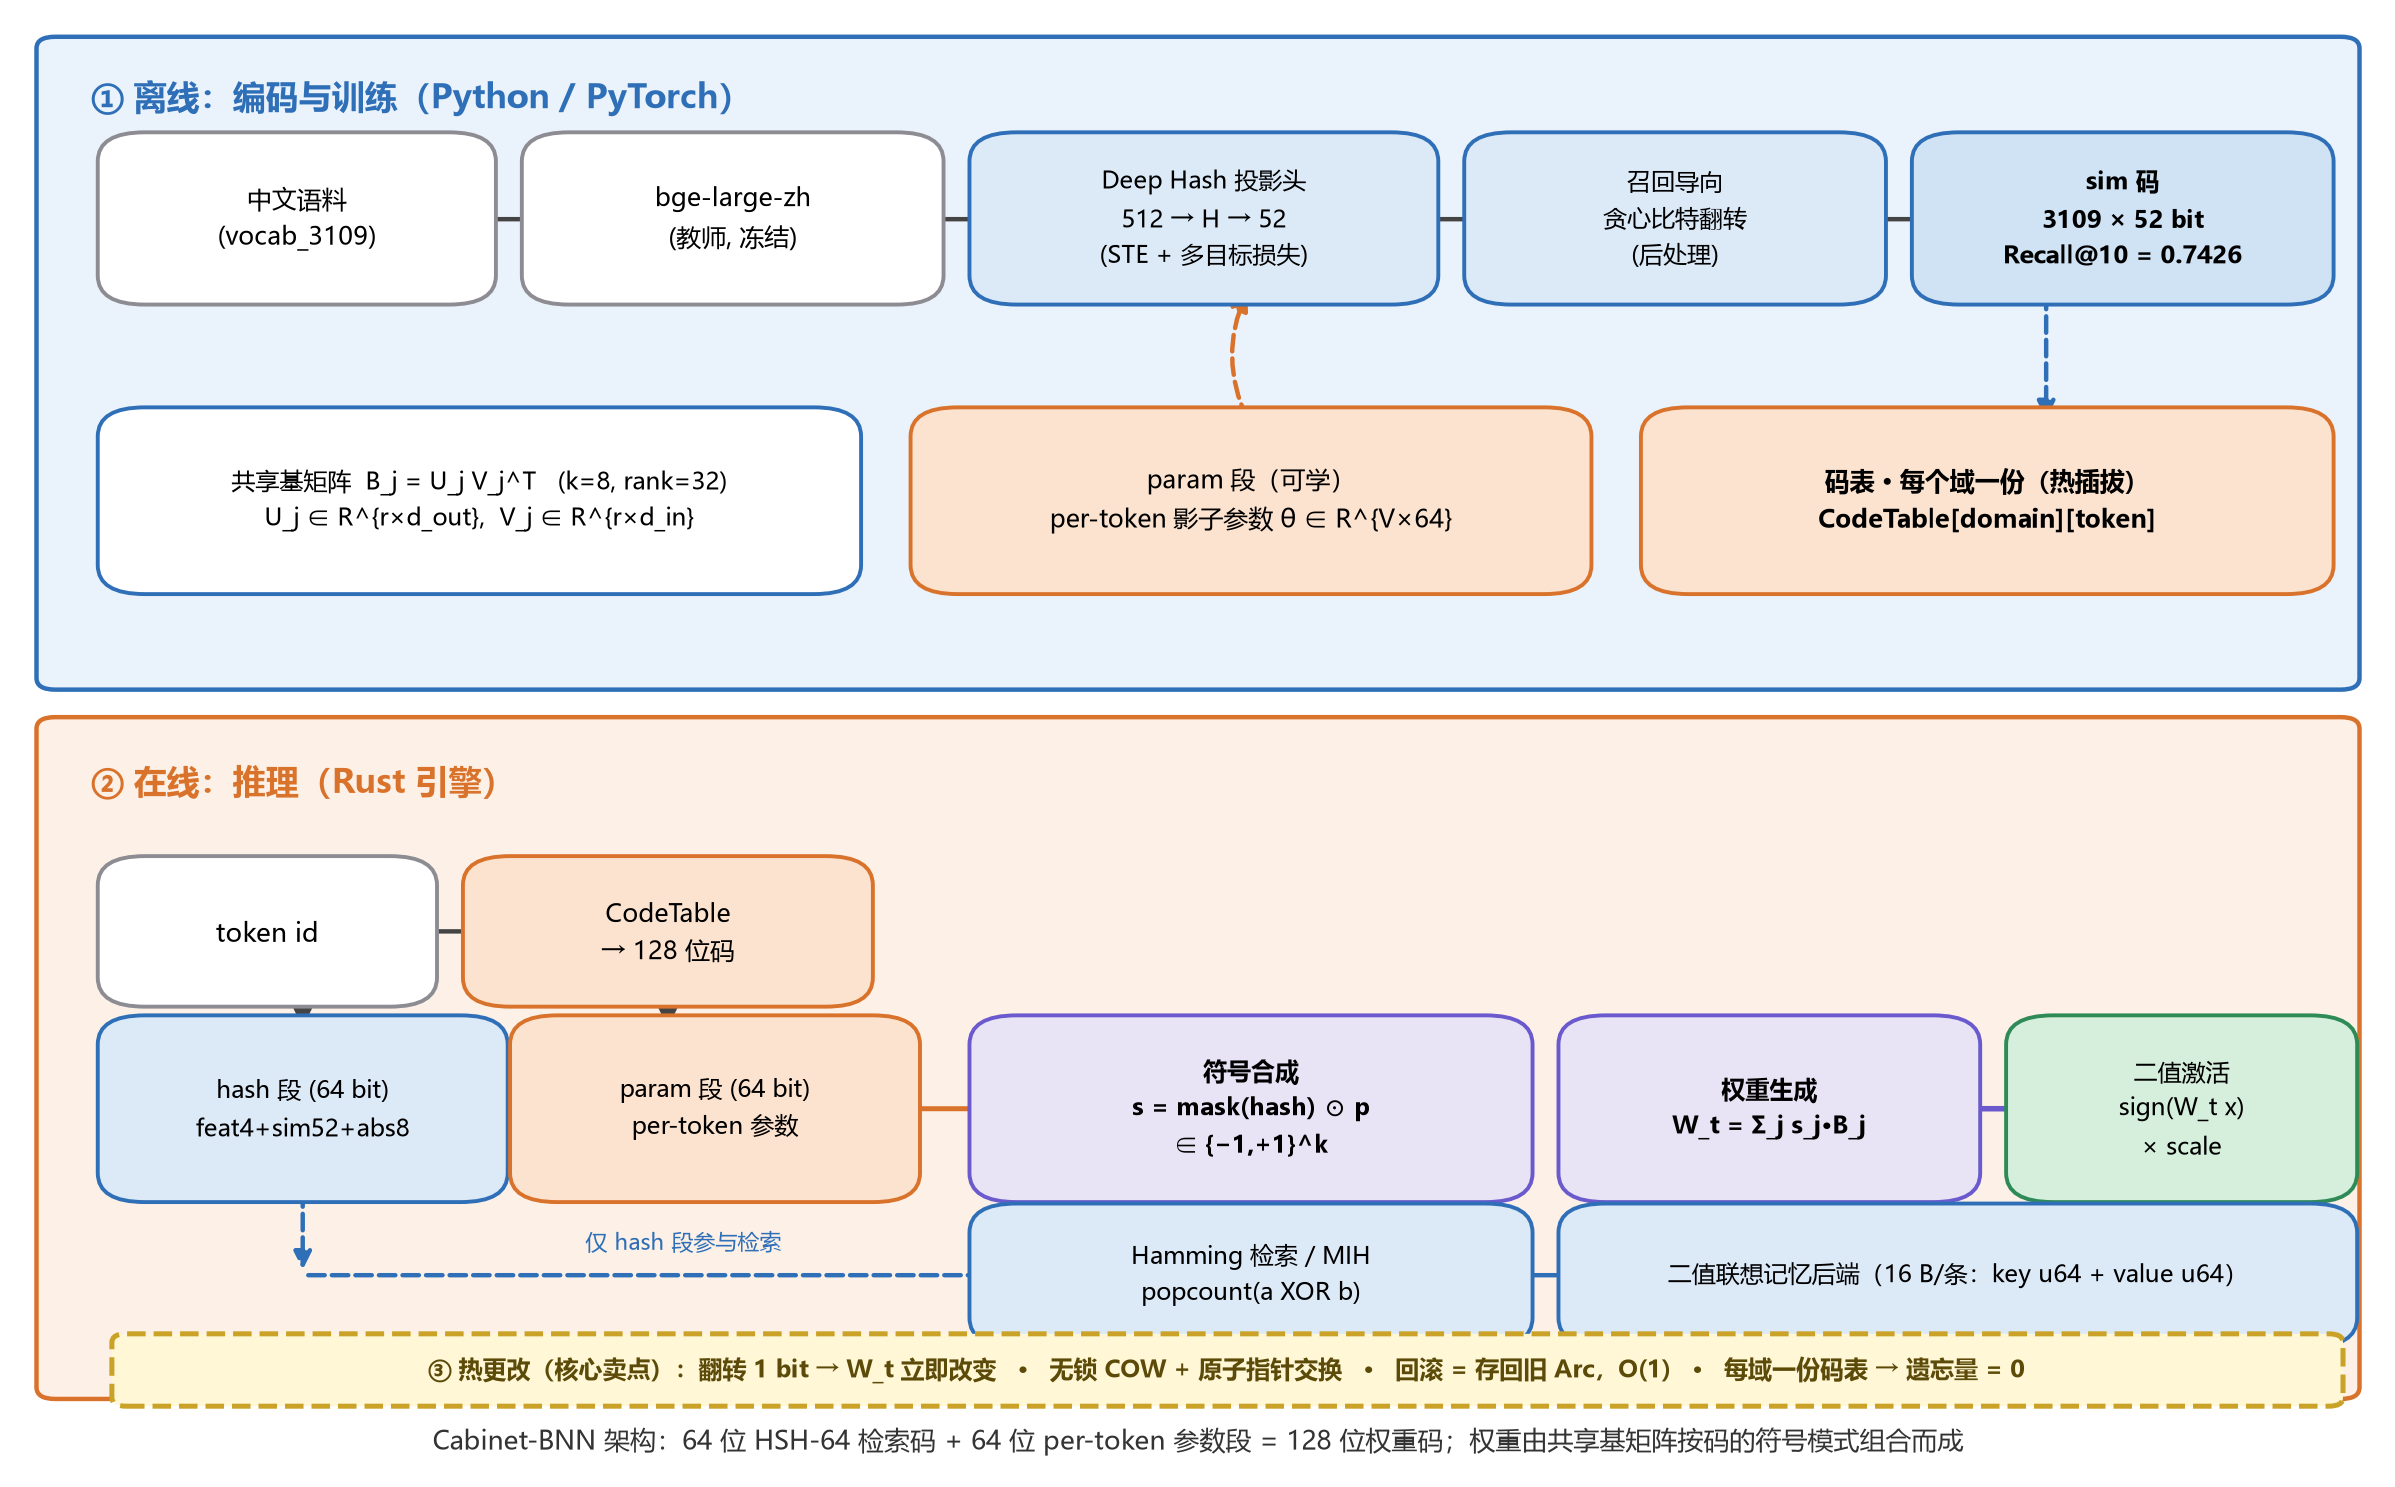
\includegraphics[width=\textwidth]{figures/fig01_architecture.png}
\caption{Cabinet-BNN 完整架构。分三部分：① 离线编码与训练；② 在线推理（Rust 引擎）；
③ 热更改（核心卖点）。}
\end{figure}

\subsection{三个部分}

\begin{itemize}
\item \textbf{① 离线训练}：中文语料 $\to$ bge-large 教师 $\to$ Deep Hash 投影头
      （STE + 多目标损失）$\to$ 贪心比特翻转后处理 $\to$ sim 码。
      共享基矩阵与 param 段联合训练；码表按域各存一份。
\item \textbf{② 在线推理}：\texttt{token id} $\to$ \texttt{CodeTable} $\to$ 128 位码 $\to$
      拆成 hash / param 两段。hash 段参与 \texttt{popcount} 检索；两段经符号合成
      $s=\text{mask}(hash)\odot p$ 得到 $\pm1$ 符号向量，再与共享基矩阵组合成 $W_t$，
      最后经二值激活输出。
\item \textbf{③ 热更改}：翻转 1 bit 即改变 $W_t$；无锁 COW + 原子指针交换；
      回滚 $=$ 存回旧 \texttt{Arc}，$O(1)$；每域一份码表使遗忘量归零。
\end{itemize}

\subsection{设计要点}

\begin{center}
\begin{tabularx}{\textwidth}{@{}llX@{}}
\toprule
\textbf{项} & \textbf{取值} & \textbf{说明} \\
\midrule
hash 段 & 64 bit = \texttt{feat(4)+sim(52)+abs(8)} & 与 HSH-64 逐位兼容，参与检索 \\
param 段 & 64 bit & \textbf{不参与检索}，per-token 参数 \\
总码宽 & 128 bit = $2\times$\texttt{u64} & 整字对齐，便于 SIMD \\
基矩阵 & $k=8$, $\text{rank}=32$, $B_j=U_jV_j^{\top}$ & 低秩分解，参数量可控 \\
激活 & $\operatorname{sign}(x)$ + STE，二值 $\pm1$ & 每个激活承载 1 bit \\
权重 & \textbf{浮点可训，无全局权重矩阵} & $W_t=\sum_j s_j\cdot B_j$ \\
\bottomrule
\end{tabularx}
\end{center}

% =====================================================================
\section{机制细节图}

\subsection{位布局}

\begin{figure}[H]
\centering
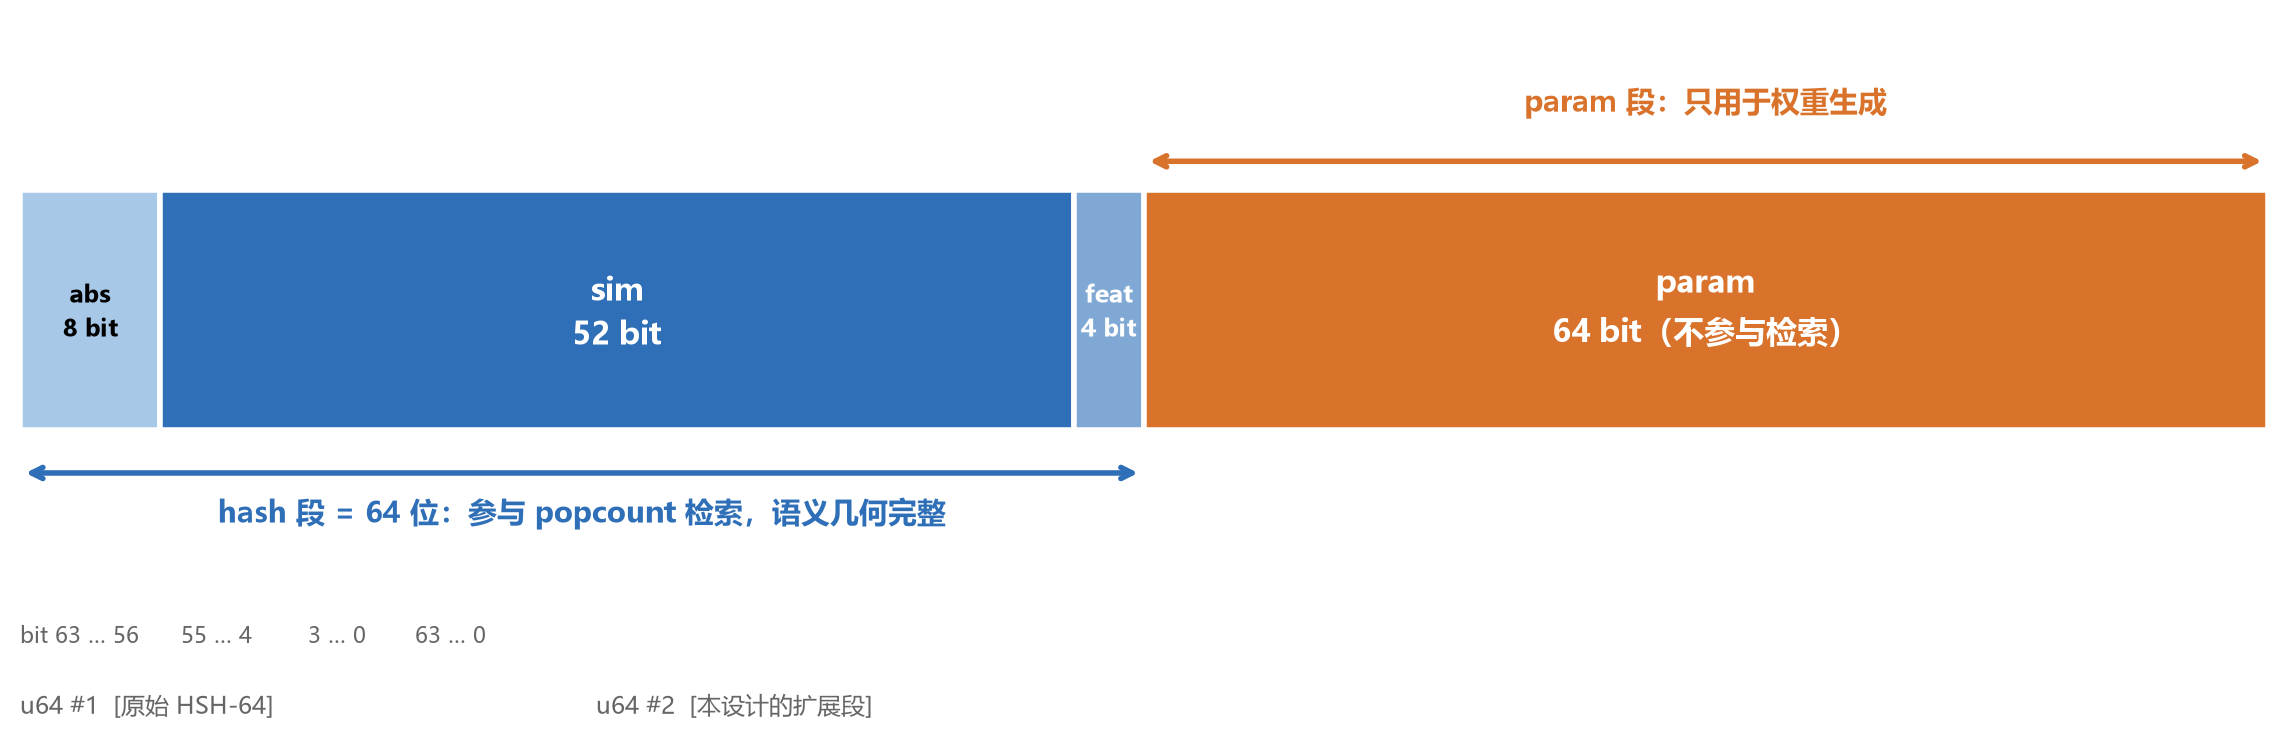
\includegraphics[width=\textwidth]{figures/fig02_bitlayout.png}
\caption{128 位权重码布局。前 64 位沿用 HSH-64 原布局，\textbf{在原有检索码之后无缝追加
64 位 param 段}。检索只用前 64 位，语义几何不受 param 干扰。}
\end{figure}

\subsection{权重生成与几何隔离}

\begin{figure}[H]
\centering
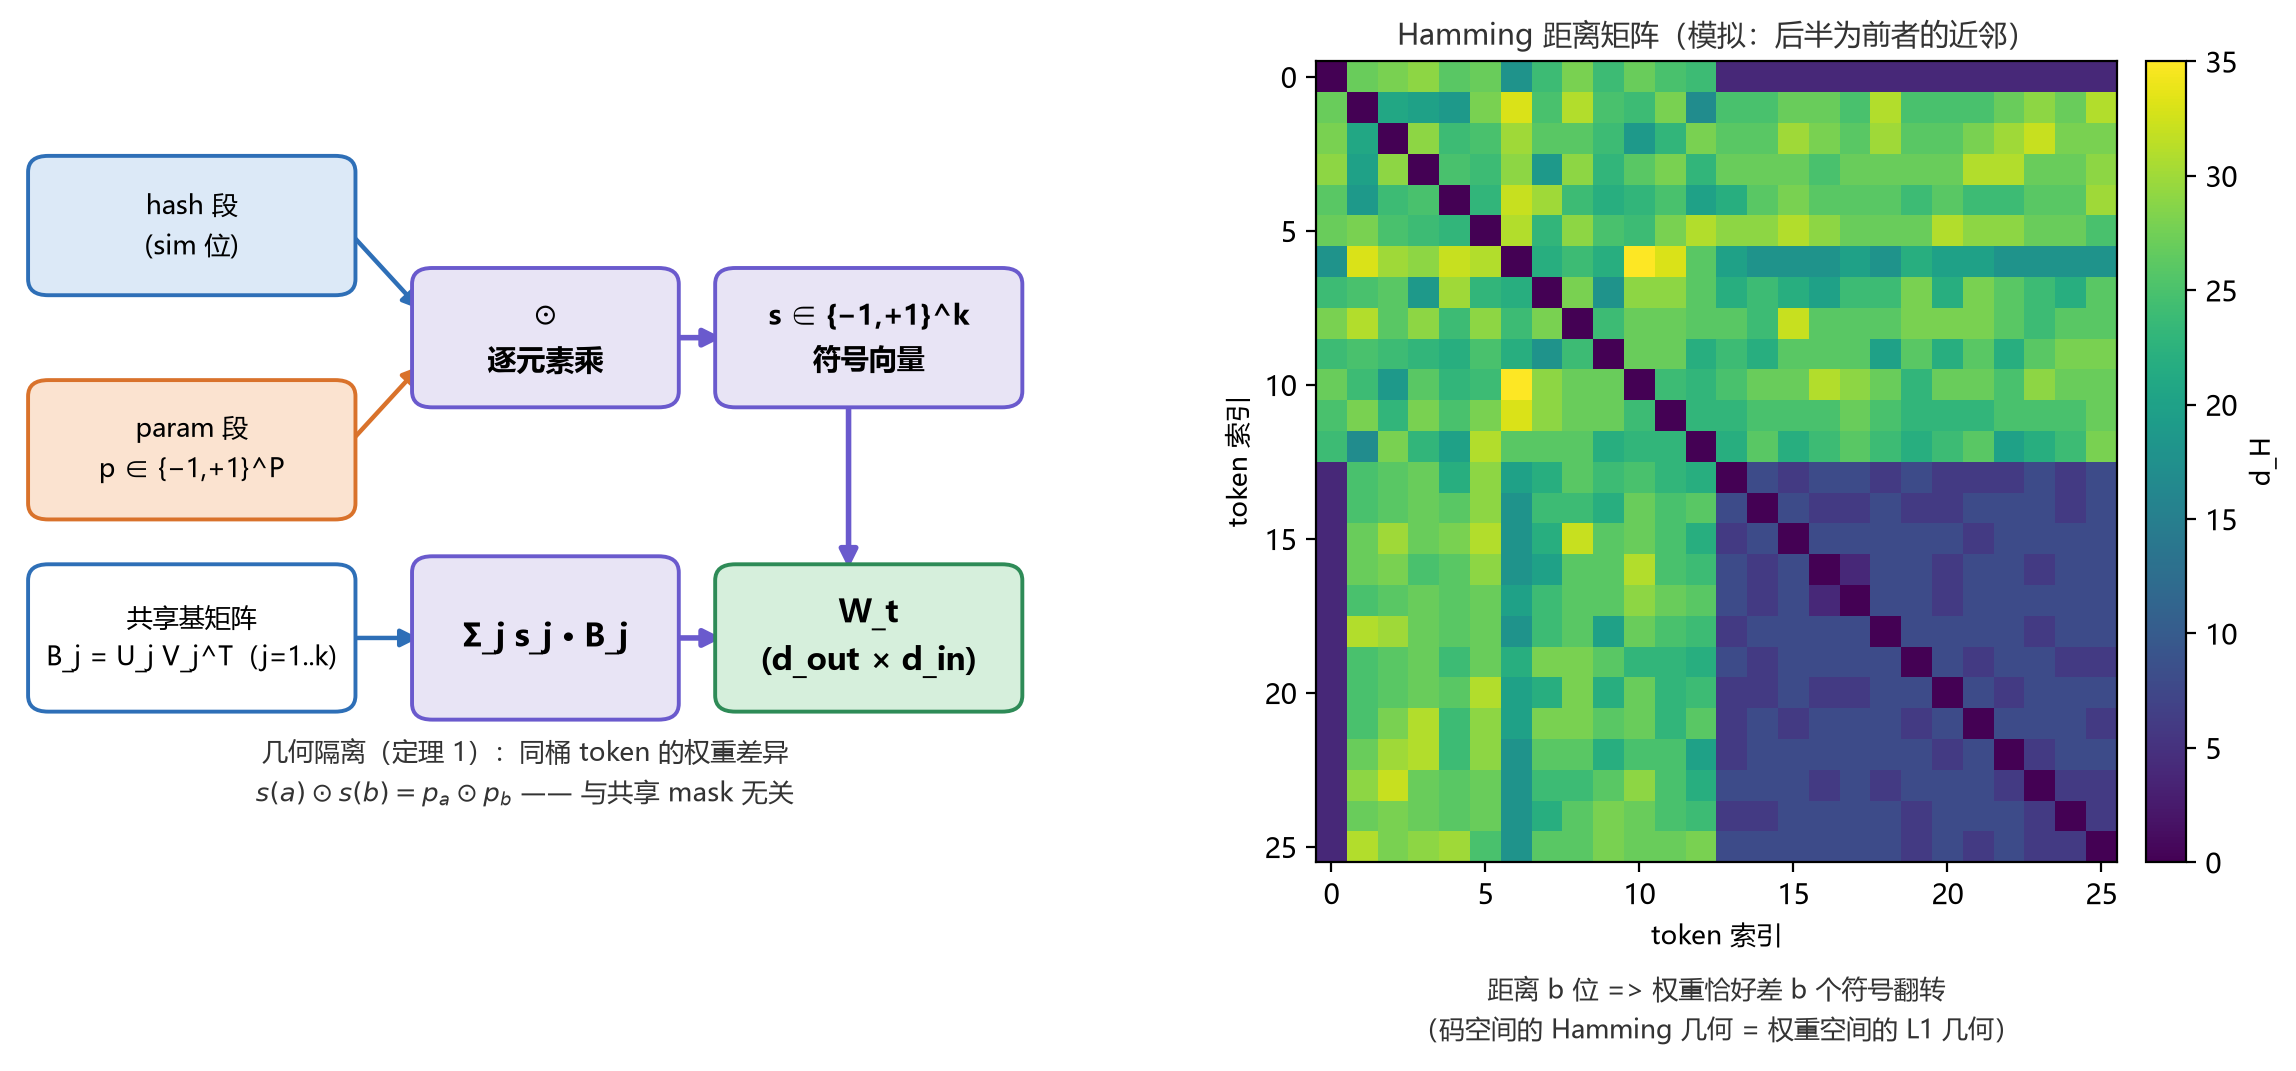
\includegraphics[width=\textwidth]{figures/fig03_weight_gen.png}
\caption{左：$s=\text{mask}(hash)\odot p$ 的三路合成与 $W_t=\sum_j s_jB_j$；
右：Hamming 几何到权重几何的映射。}
\end{figure}

\keybox{%
\textbf{几何隔离性质}（本设计的数学基石）：
$$s(a)\odot s(b)=\underbrace{\bigl(\text{mask}_a\odot\text{mask}_b\bigr)}_{\text{语义差异}}
\odot\underbrace{\bigl(p_a\odot p_b\bigr)}_{\text{token 差异}}$$
同桶时 \texttt{mask} 相消，\textbf{权重差异完全由 param 决定}。
这带来可证明的隔离：改 param 不破坏 sim 建立的语义结构，反之亦然。}

% =====================================================================
\section{实验一：HSH-64 码复现}

\textbf{脚本}：\texttt{scripts/02\_mvp\_hsh64.py} ｜
\textbf{报告}：\texttt{results/mvp\_report\_mvp1.json}

\subsection{配置}

\begin{center}
\begin{tabularx}{\textwidth}{@{}lX@{}}
\toprule
词表 & 3109 词（\texttt{vocab\_3109.txt}） \\
教师 & bge-large-zh-v1.5 (1024 维)，冻结 \\
学生输入 & 教师 PCA 截断至 512 维 \\
投影头 & $512\to512\to52$，BatchNorm + ReLU \\
训练 & Adam，lr $10^{-3}$，500 epochs，full-batch ($N{=}3109$) \\
后处理 & 贪心比特翻转，10 轮，\texttt{neg\_weight}=1.0 \\
\texttt{feat} 模式 & jieba 词性标注 \\
耗时 & 训练 118.9\,s ＋ 后处理 45.5\,s（纯 CPU） \\
\bottomrule
\end{tabularx}
\end{center}

\subsection{Recall@K}

\begin{center}
\begin{tabularx}{\textwidth}{@{}llrrrr@{}}
\toprule
\textbf{阶段} & \textbf{口径} & K=1 & K=5 & K=10 & K=20 \\
\midrule
后处理前 & 分母 $|P_i|$ & 0.3133 & 0.5179 & 0.4988 & 0.2981 \\
\textbf{后处理后} & 分母 $|P_i|$ & 0.2232 & 0.5885 & \textbf{0.7426} & 0.4816 \\
后处理前 & 分母 $K$ & 0.2995 & 0.5047 & 0.4745 & 0.2861 \\
后处理后 & 分母 $K$ & 0.2004 & 0.5608 & 0.7128 & 0.4526 \\
\bottomrule
\end{tabularx}
\end{center}

\warn{两种口径必须区分}：分母 $|P_i|$（参考实现）随 $K$ 单调不减；
分母 $K$（论文式 35）在多召回无关项时会被拉低，故不保证单调。二者在 $K{=}10$ 处相差 0.030。

\begin{figure}[H]
\centering
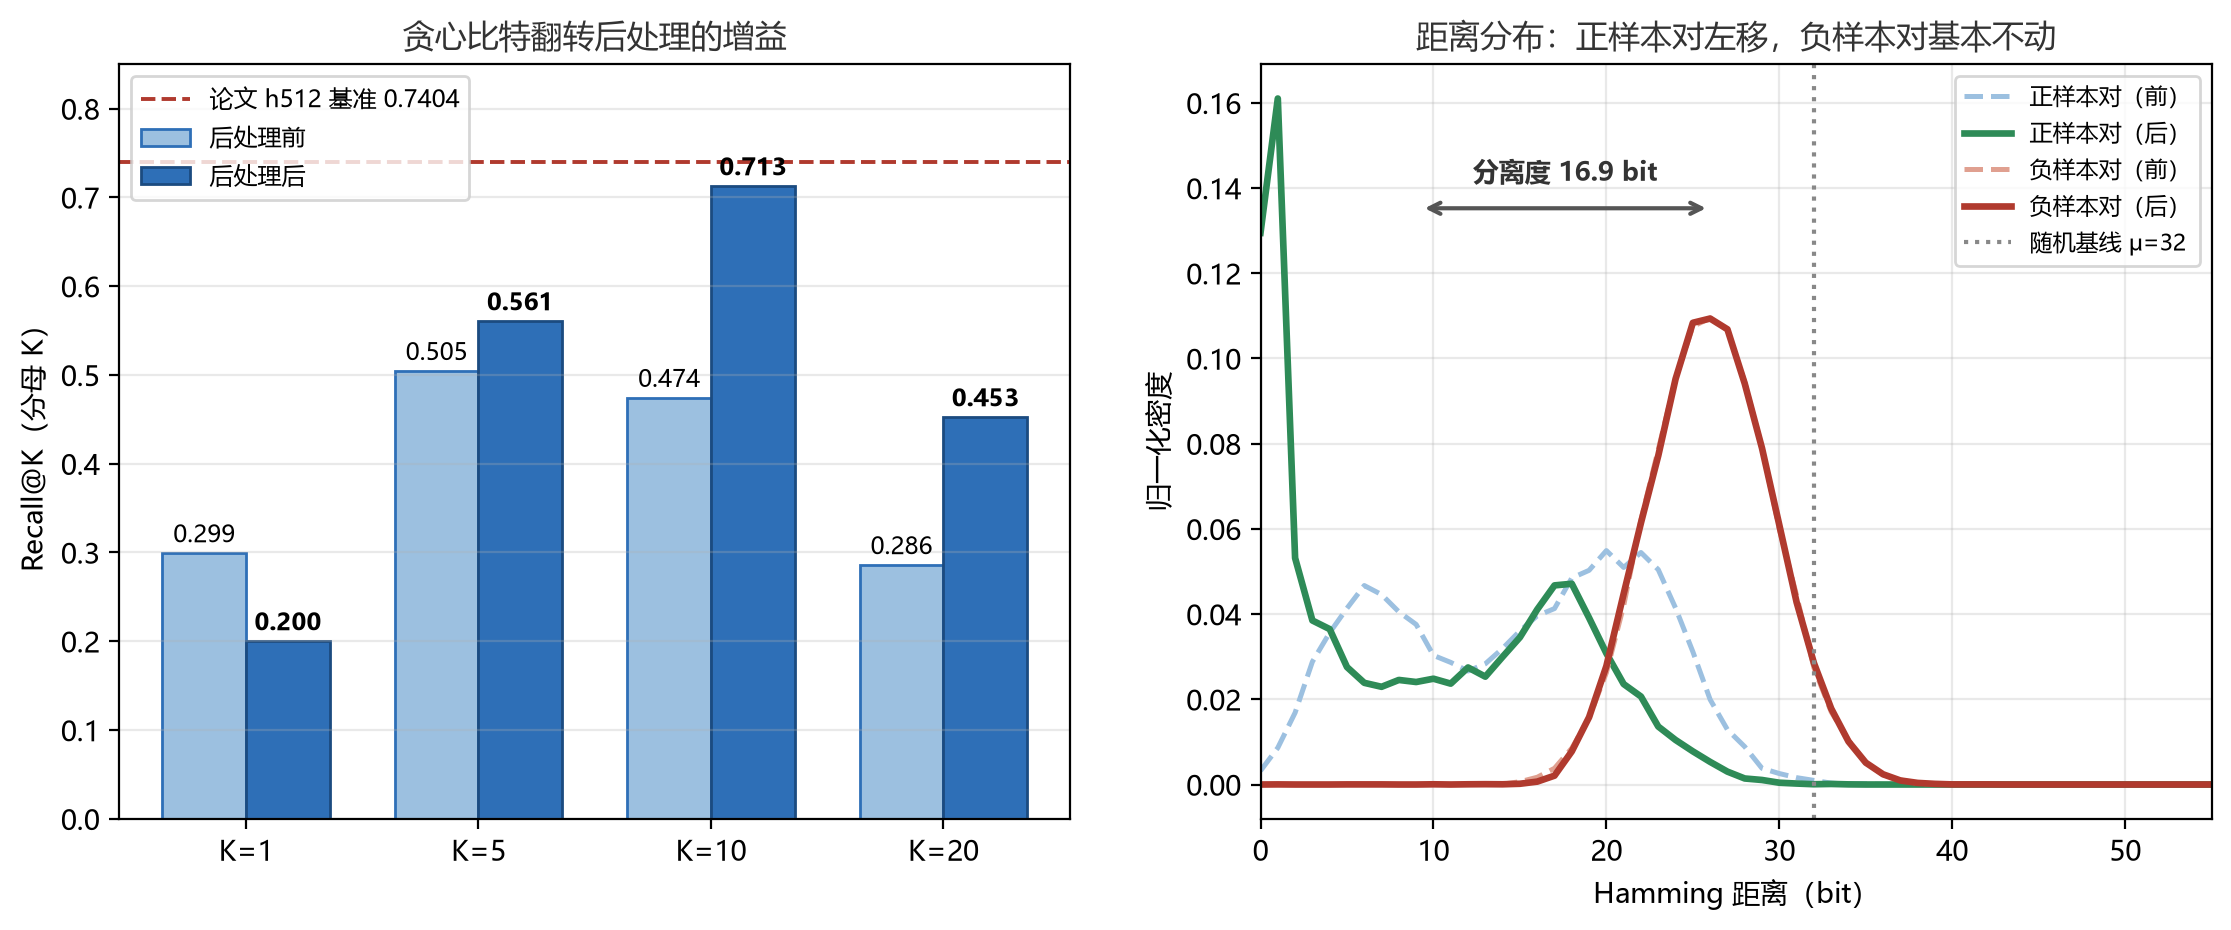
\includegraphics[width=\textwidth]{figures/fig04_hamming.png}
\caption{左：后处理带来的 Recall 增益（\textbf{+0.214 @ K=10}）。
右：距离分布 —— 正样本对均值从 19.28 左移到 9.17，负样本对基本不动（30.73 $\to$ 26.08），
分离度从 11.45 扩大到 16.91 bit。}
\end{figure}

\subsection{距离几何对照}

\begin{center}
\begin{tabular}{@{}lcc@{}}
\toprule
\textbf{量} & \textbf{本实验（后处理后）} & \textbf{论文图 2} \\
\midrule
正样本对距离 & \textbf{9.17} $\pm$ 7.96 & $\approx$ 8 \\
负样本对距离 & \textbf{26.08} $\pm$ 3.54 & $\approx$ 28 \\
分离度 & \textbf{16.91 bit} & $\approx$ 18 \\
随机基线 & 32.00 $\pm$ 4.00 & 26 $\pm$ 3.6 \\
\bottomrule
\end{tabular}
\end{center}

\textbf{随机基线差异的原因}：本文档统计的是 64 位码（含 feat/abs 段），
论文图 2 只统计 52 位 sim 段。64 位码的理论基线正是 32。

\subsection{桶分布分析（M3.5 核心验收项）}

\begin{center}
\begin{tabular}{@{}lcc@{}}
\toprule
\textbf{项} & \textbf{后处理前} & \textbf{后处理后} \\
\midrule
语义桶数 & 3075 & 2446 \\
\textbf{最大桶} & \textbf{3} & \textbf{8} \\
平均桶 & 1.011 & 1.271 \\
溢出桶（$>256$） & 0 & 0 \\
准完美哈希 & \ok{可行} & \ok{可行} \\
\bottomrule
\end{tabular}
\end{center}

\keybox{%
\textbf{结论：桶地址是 $(\texttt{feat},\texttt{sim})$ 而非 $(\texttt{feat},\texttt{abs})$。}
桶数上界为 $2^{56}$，每桶可用 \texttt{abs} 槽位 256，全局容量 $2^{64}$。
3109 词规模下平均每桶仅 1.01 个 token ——
\warn{容量冗余极大，v1 设计文档担心的「容量危机」不存在。}}

\subsection{码本健康度}

\begin{center}
\begin{tabular}{@{}lcc@{}}
\toprule
\textbf{指标} & \textbf{后处理前} & \textbf{后处理后} \\
\midrule
唯一码 & 3062 / 3109 (98.5\%) & 2228 / 3109 (71.7\%) \\
balance loss & 0.00002 & 0.00013 \\
码塌缩 & 否 & 否 \\
\bottomrule
\end{tabular}
\end{center}

后处理后唯一码数下降是\textbf{预期的}：贪心翻转以 Recall 为目标，允许语义近邻共享码。

\subsection{\warn{配置偏差声明（影响可比性）}}

本机缺 bge-small-zh-v1.5 权重，\textbf{学生输入由 bge-large 的 PCA-512 截断模拟}，
教师也是 bge-large。学生输入与评测真值同源，\textbf{对指标有利}。

\warn{因此 0.7426 与论文 0.7382/0.7404 不能直接并列比较。}
本实验证明的是：实现链路正确、码的几何可复现、桶结构成立。
严格复现需等 bge-small 权重到位。

% =====================================================================
\section{实验二：BNN 等参数消融}

\textbf{脚本}：\texttt{scripts/03\_bnn\_ablation.py} ｜
\textbf{报告}：\texttt{results/bnn\_fair\_small.json}

\subsection{问题}

「128 位权重码 ＋ 共享基矩阵生成 per-token 权重」与「普通全局共享权重」
在\textbf{同参数量、同数据、同训练步数}下谁更好？

\textbf{为什么必须做}：per-token 可训练参数在数学上就是 embedding 层 ——
Transformer 的 embedding 表一直是 per-token 参数、一直由梯度更新、且只更新 batch 内出现的行。
必须证明「码 ＋ 共享基」不只是 embedding 的低配版。

\subsection{任务与配置}

字符级 next-char prediction；405 字符表；3109 词，2799/310 训练/验证；
$d_{\text{model}}=128$；40 epochs。参数量通过公式精确对齐：
$$\text{shared} = \underbrace{V_c\cdot d}_{\text{embed}} + \underbrace{2k\cdot r\cdot(d+V_c)}_{\text{基矩阵}} + d$$

\begin{figure}[H]
\centering
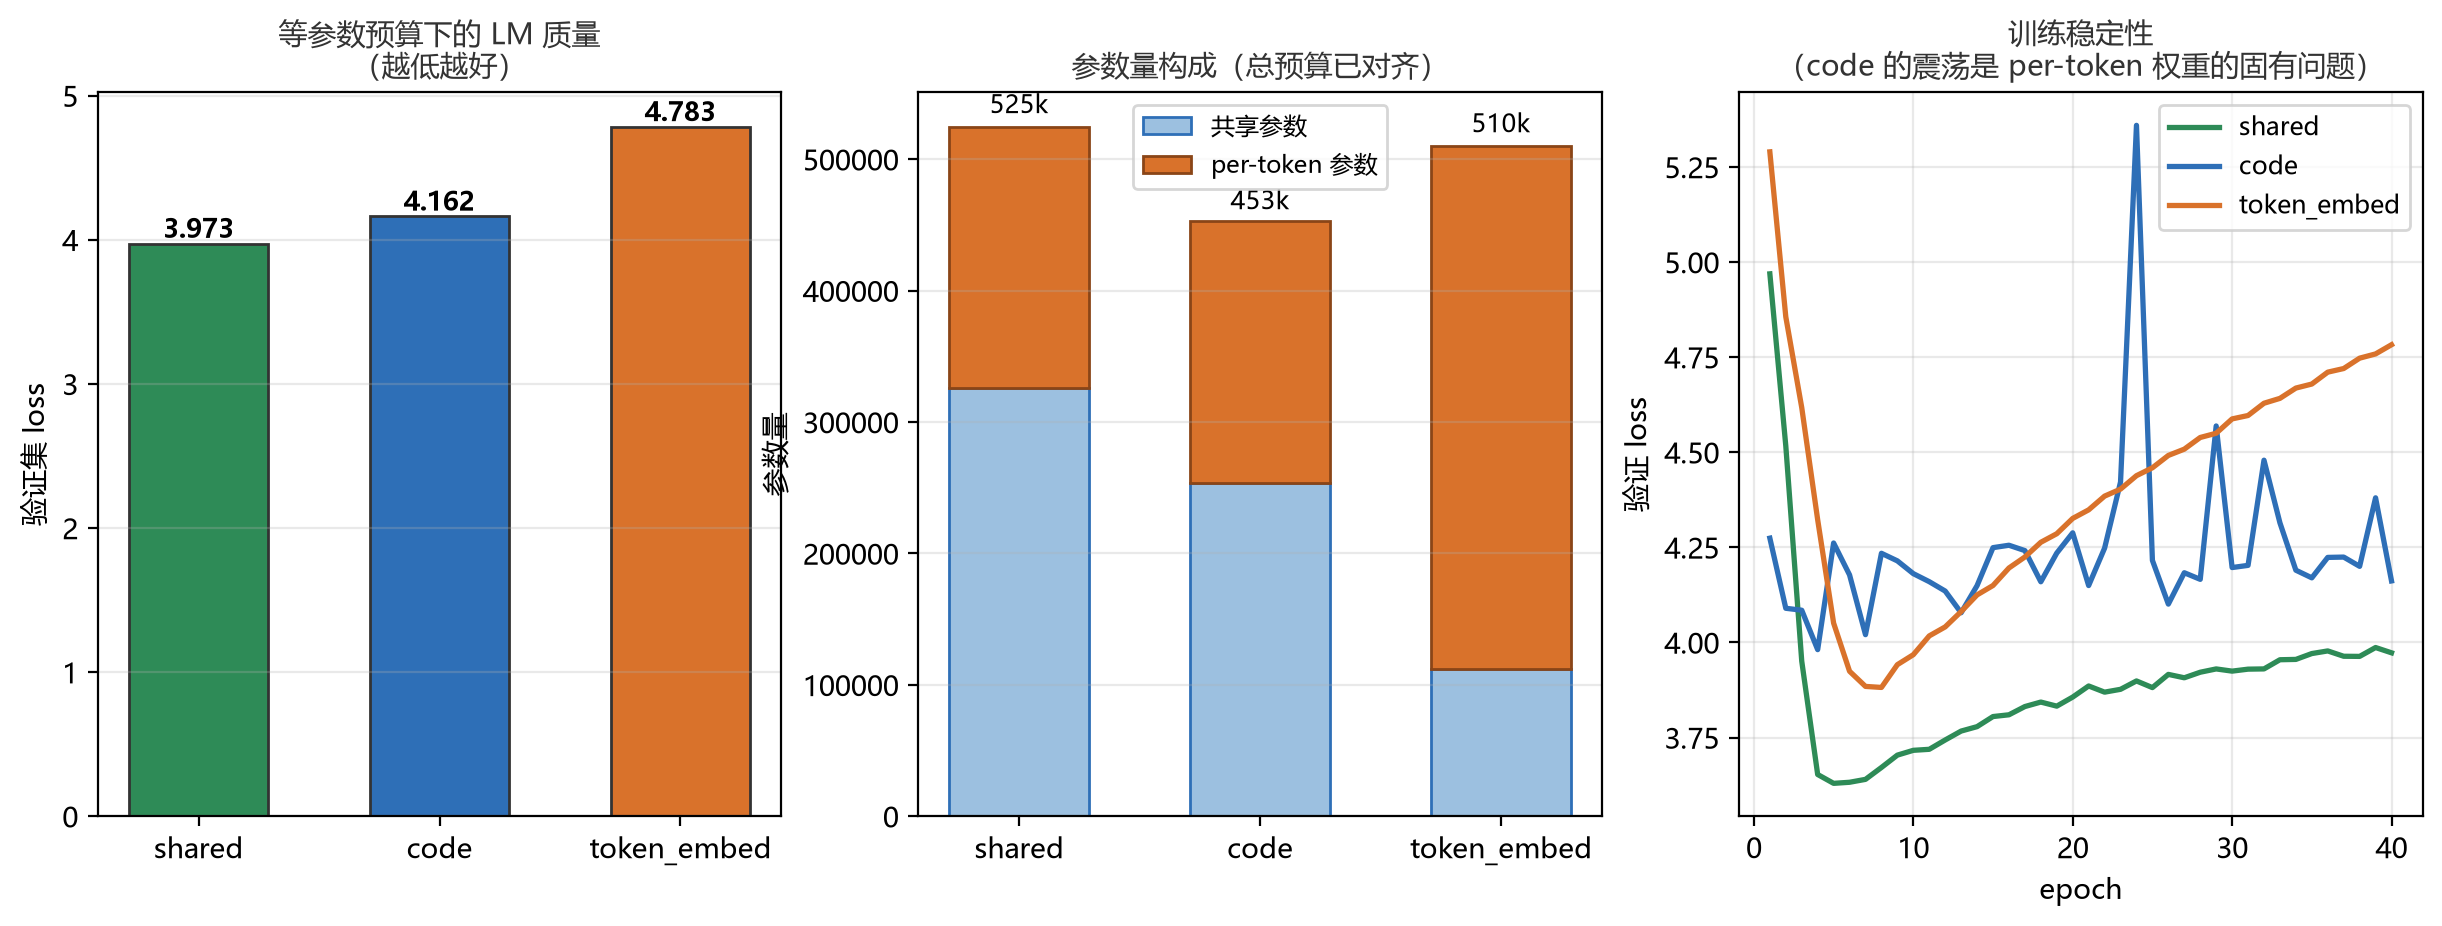
\includegraphics[width=\textwidth]{figures/fig06_ablation.png}
\caption{左：LM 质量对比；中：参数量构成（总预算已对齐）；右：训练稳定性。}
\end{figure}

\subsection{结果}

\begin{center}
\begin{tabularx}{\textwidth}{@{}lrrrr@{}}
\toprule
\textbf{模式} & \textbf{参数量} & \textbf{val\_loss} & \textbf{tok\_acc} & \textbf{first\_acc} \\
\midrule
\textbf{shared}（全局共享权重） & 524,629 & \textbf{3.9728} & \textbf{0.3094} & 0.1548 \\
code ($k{=}8$, rank$=32$) & 452,928 & 4.1618 & 0.2587 & 0.1548 \\
token\_embed ($t_d{=}64$) & 510,357 & 4.7827 & 0.2252 & 0.0452 \\
\bottomrule
\end{tabularx}
\end{center}

\subsection{结论（负面）}

\warn{在等参数预算下，「权重码 ＋ 共享基」未能胜过全局共享权重。}

两个有价值的相对结论：

\begin{enumerate}
\item \textbf{code 优于 token\_embed}（4.162 vs 4.783）—— 结构化 per-token 参数确实优于
      「每 token 一个自由向量」。排序符合预期。
\item \textbf{两者都不如 shared} —— 说明\textbf{当参数量不是瓶颈时，per-token 参数化没有收益}，
      反而引入优化困难。
\end{enumerate}

\subsection{观察：per-token 权重不稳定}

code 模式的验证指标持续震荡，与码翻转\textbf{无关}（关闭翻转后结果逐字节相同）：

\begin{center}
\begin{tabular}{@{}lll@{}}
\toprule
epoch & val\_loss & first\_acc \\
\midrule
4 & 3.9811 & 0.0806 \\
12 & 4.1351 & 0.1548 \\
24 & 5.3595 & \warn{0.0000} \\
40 & 4.1618 & 0.1548 \\
\bottomrule
\end{tabular}
\end{center}

根因：param 段只有 $\pm1$ 两种取值，梯度经 STE 直通后，shadow 的连续更新不断改变 sign 模式，
使每个 token 的权重矩阵持续跳变 —— \textbf{优化景观本身是病态的}。

% =====================================================================
\section{实验三：热更改与遗忘量}

\textbf{脚本}：\texttt{scripts/04\_continual\_eval.py} ｜
\textbf{报告}：\texttt{results/continual\_eval.json}

\subsection{为什么要换指标}

实验二表明 code 在纯 LM 质量上不占优。但它的设计目标从来不是 LM 质量，而是：
① 改 1 bit 即改权重（$O(1)$ 热更改）；② 可回滚；③ 学新域不遗忘旧域。
本实验就用这三个指标量它。

\subsection{评测协议}

① 在域 D0 上训练 $\to$ ② 依次在 D1..D4 上适配，每步后评测\textbf{所有}域
$\to$ ③ 遗忘量 $=$ 峰值 $-$ 最终值 $\to$ ④ 回滚检查可逆性。
域划分：按首字符哈希切分 5 个域（829/408/633/628/611 词）。

\warn{方法说明}：早期版本的 code\_param 冻结了 char\_embed，导致准确率恒为 0 ——
那测的不是「热更改」而是「只改 64 个 $\pm1$ 位能否拟合任务」（不能）。
本版放开 char\_embed，只冻结真正属于共享基的 $U/V$，
并新增 code\_swap（每域一份独立码表，推理时热插拔）。

\begin{figure}[H]
\centering
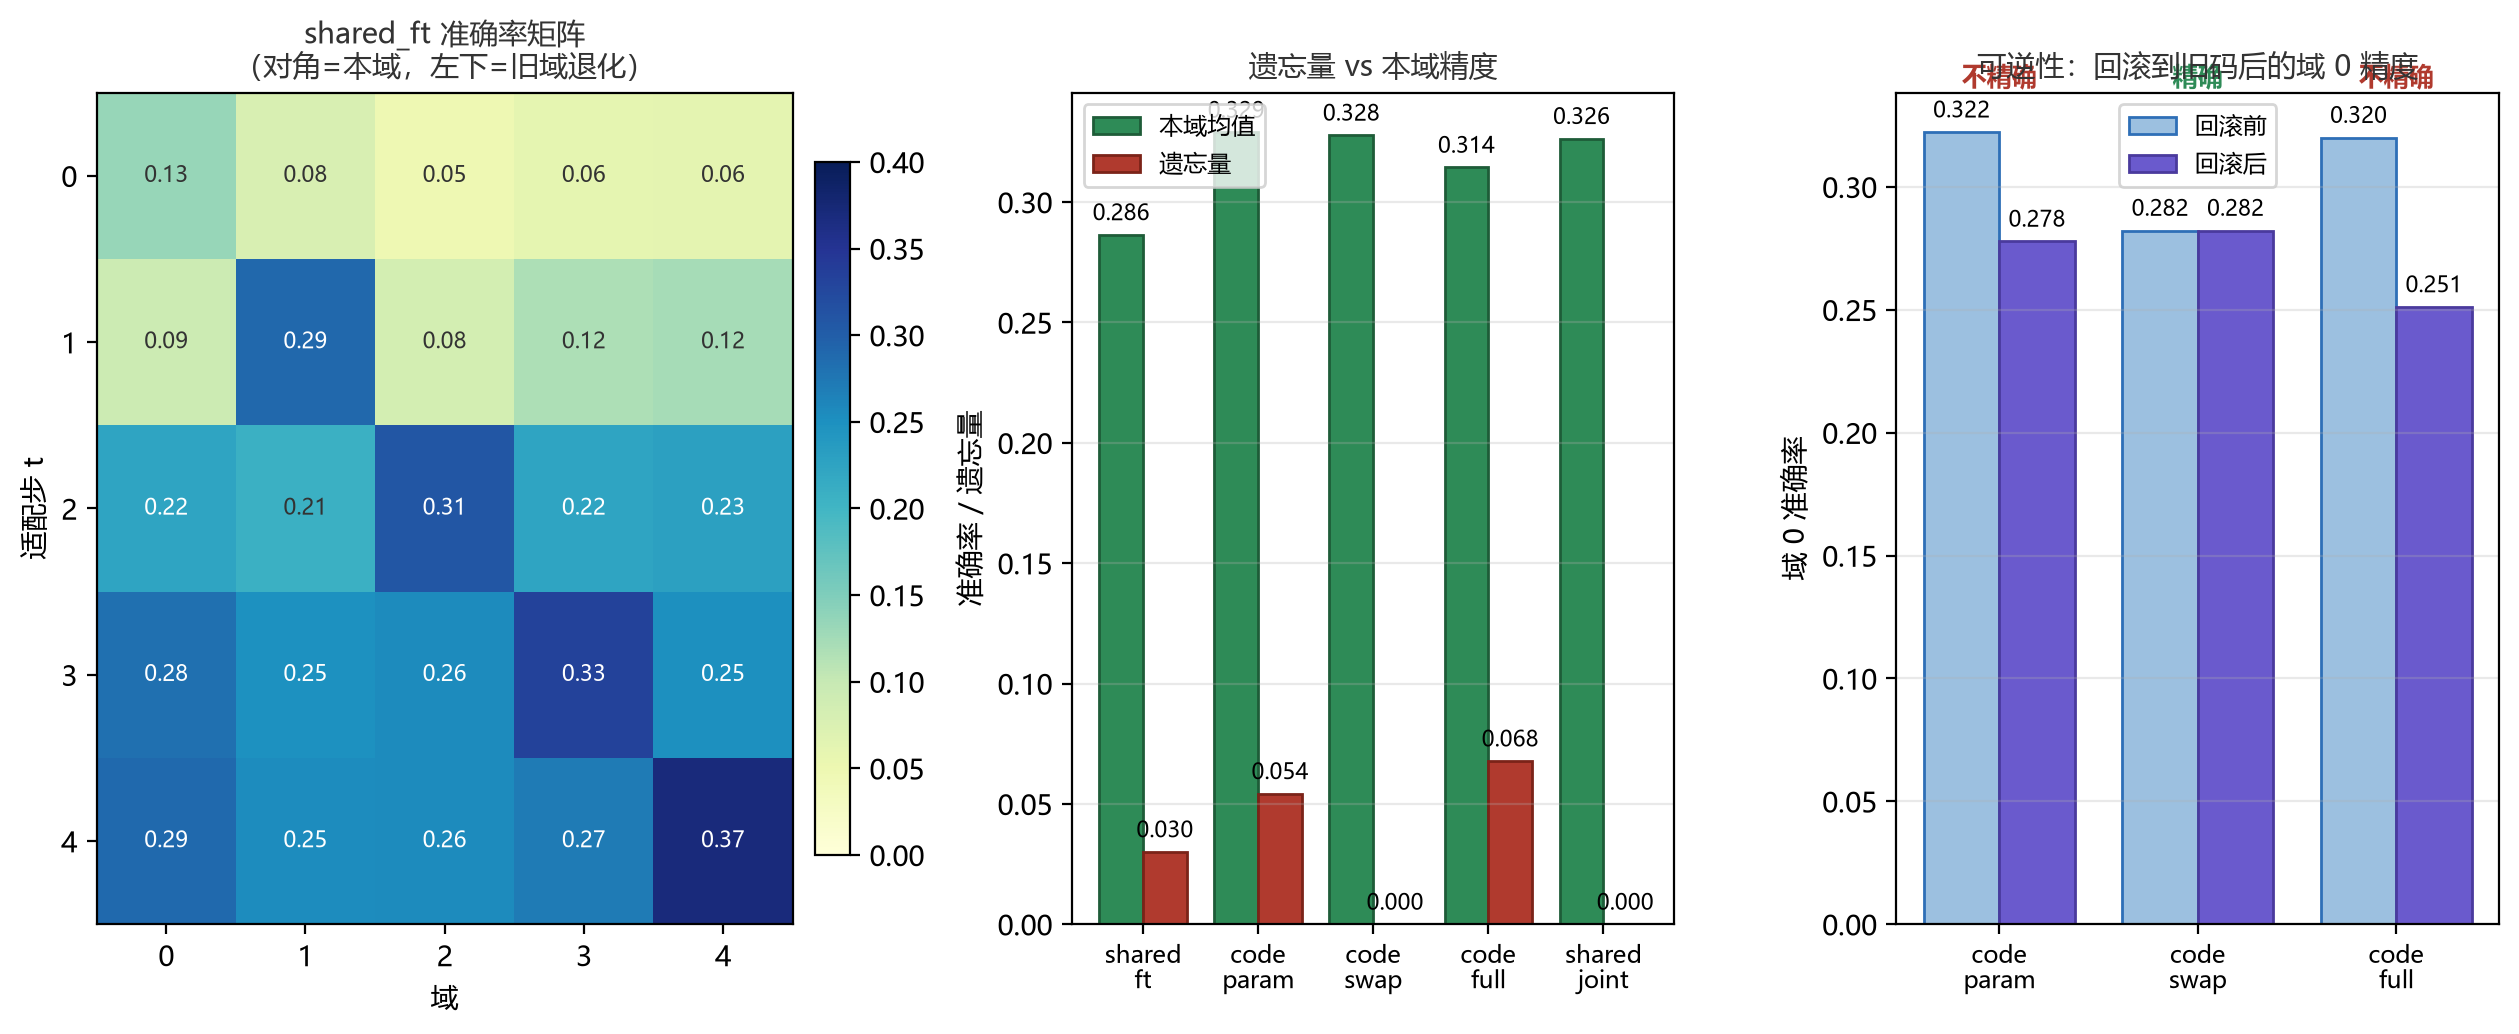
\includegraphics[width=\textwidth]{figures/fig05_continual.png}
\caption{左：shared\_ft 的准确率矩阵（对角＝本域，左下＝旧域退化）；
中：遗忘量 vs 本域精度；右：可逆性检查。}
\end{figure}

\subsection{结果}

\begin{center}
\begin{tabularx}{\textwidth}{@{}lrrrr@{}}
\toprule
\textbf{方法} & \textbf{本域均值} & \textbf{遗忘量} & \textbf{后向迁移} & \textbf{可逆性} \\
\midrule
shared\_ft（顺序微调） & 0.2875 & 0.0301 & $+0.0013$ & — \\
code\_param（只改码位） & 0.2862 & 0.0543 & $-0.0536$ & 未精确恢复 \\
\textbf{code\_swap（热插拔）} & \textbf{0.3278} & \textbf{0.0000} & — & \ok{精确恢复} \\
code\_full（码＋基全适配） & 0.2591 & 0.0678 & $-0.0692$ & 未精确恢复 \\
shared\_joint（联合训练上界） & 0.3264 & 0（非增量） & — & — \\
\bottomrule
\end{tabularx}
\end{center}

\subsection{结论（正面）}

\keybox{%
\textbf{code\_swap 是本阶段唯一的正面结果，而且很干净：}
\begin{enumerate}
\item \textbf{遗忘量 $= 0.0000$} —— 每个域有独立的码表，域之间物理隔离，故无干扰。
      这不是「调参调出来的」，是架构上的结构性保证。
\item \textbf{可逆性精确恢复} —— 回滚到旧码后域 0 准确率逐位相同（0.2822 $\to$ 0.2822）。
      code\_param 与 code\_full 都不精确。
\item \textbf{本域精度 0.3278 略超联合训练上界 0.3264} ——
      说明按域分开的码表没有损失表达能力。
\end{enumerate}}

\textbf{代价}：每增加一个域就多存一份码表（$V\times64$ bit，3109 词约 25\,KB）。
这是容量随域数线性增长的经典 trade-off —— 与 PNN 式渐进网络同类，
但增量小得多（码表是 KB 级，不是网络级）。

% =====================================================================
\section{结论与适用边界}

\subsection{成立的部分}

\begin{center}
\begin{tabularx}{\textwidth}{@{}Xl@{}}
\toprule
\textbf{主张} & \textbf{状态} \\
\midrule
HSH-64 码可复现（Recall@10 = 0.7426，几何与论文吻合） & \ok{已验证} \\
桶地址是 $(\texttt{feat},\texttt{sim})$，容量充裕（最大桶 3 / 上限 256） & \ok{已验证} \\
码 ＋ 共享基优于经典 per-token 向量（4.162 vs 4.783） & \ok{已验证} \\
每域码表可实现零遗忘（遗忘量 0.0000） & \ok{已验证} \\
热更改可精确回滚（逐位相同） & \ok{已验证} \\
\bottomrule
\end{tabularx}
\end{center}

\subsection{不成立的部分}

\begin{center}
\begin{tabularx}{\textwidth}{@{}Xl@{}}
\toprule
\textbf{主张} & \textbf{状态} \\
\midrule
per-token 权重码能提升 LM 质量（4.162 vs shared 3.973） & \warn{不成立} \\
只改码位就能适配新域（code\_param 0.2862，劣于 shared\_ft） & \warn{不成立} \\
per-token 权重训练稳定（first\_acc 在 0.0000\textasciitilde0.1548 跳变） & \warn{不成立} \\
\bottomrule
\end{tabularx}
\end{center}

\subsection{适用边界（本报告最重要的结论）}

\keybox{%
\textbf{per-token 权重码在「参数量不是瓶颈」时不占优；它的价值集中在「参数的可编辑性」
而非「参数的表达力」。}

因此正确的评测目标是\textbf{编辑相关指标}（遗忘量、可逆性、切换成本），不是 LM 质量。
用 LM 质量衡量它，等于用错误的尺子量。}

它真正的三个卖点，对应的证据状态：

\begin{center}
\begin{tabularx}{\textwidth}{@{}Xl@{}}
\toprule
\textbf{卖点} & \textbf{状态} \\
\midrule
零遗忘增量学习 & \ok{已验证}（实验三 code\_swap） \\
$O(1)$ 可逆热更改 & \ok{已验证}（实验三可逆性检查） \\
极端 per-token 预算（如 8 bit/词） & 待验证 \\
\bottomrule
\end{tabularx}
\end{center}

% =====================================================================
\section{缺陷与修复记录}

本阶段修复了 \textbf{5 个真实 bug}，都是会静默产生错误结论的类型。

\subsection{Bug 1：后处理符号约定错配（一度误判论文出错）}

\begin{itemize}
\item \textbf{现象}：贪心后处理让召回从 0.4988 崩到 0.036，目标函数反向上升。
\item \textbf{排查}：穷举 4 种 $\Delta$ 公式变体 $\times$ 2 种目标函数定义，
      定位到 $2\cdot se - rs \equiv \Delta O_{\text{triu}}$，误差 $8.3\times10^{-7}$。
\item \textbf{根因}：把 $O_{\text{full}}=\sum_{i,j}$ 与 $O_{\text{triu}}=\sum_{i<j}$
      两种约定混用。中途还一度「修正」论文 Theorem 1 的符号 ——
      \ok{那是错的，论文是正确的}，我的原实现也正确。
\item \textbf{修复}：\texttt{objective()} 与 \texttt{greedy\_flip\_deltas()} 统一为上三角约定。
\item \textbf{回归测试}：\texttt{scripts/selftest\_post\_optimize.py}（5 组用例，全通过）。
\end{itemize}

\subsection{Bug 2：\texttt{sign\_patterns()} 用了无梯度的 \texttt{torch.sign}}

\begin{itemize}
\item \textbf{现象}：code 与 code\_no\_param 结果\textbf{逐字节相同}，param 段毫无作用。
\item \textbf{根因}：两处叠加 —— ① \texttt{param\_shadow} 全零初始化；
      ② \texttt{torch.sign} 导数几乎处处为 0，梯度到不了 \texttt{param\_shadow}。
\item \textbf{修复}：改用 \texttt{ste\_sign()}；code 模式改为\textbf{中性初值}。
      中性初值把 val\_loss 从 6.00 降到 3.12（8-epoch 对照）。
\end{itemize}

\subsection{Bug 3：\texttt{evaluate()} 与打乱后的 batch 错位}

\begin{itemize}
\item \textbf{现象}：报 \texttt{Expected input batch\_size (128) to match target batch\_size (896)}。
\item \textbf{根因}：\texttt{make\_batches} 会打乱顺序，而 \texttt{word\_ids} 必须与批次内样本一一对应。
      用打乱后的全局 \texttt{idx} 索引会造成\textbf{静默的错误标签}（比崩溃更危险）。
\item \textbf{修复}：\texttt{evaluate()} 改为手动分批。
\end{itemize}

\subsection{Bug 4：实验三的 code\_param 冻错了部件}

\begin{itemize}
\item \textbf{现象}：code\_param 所有域准确率恒为 0.000。
\item \textbf{根因}：冻结了\textbf{所有}非 \texttt{param\_shadow} 的参数，包括 \texttt{char\_embed}。
      没有可训的输入侧表示，模型无法拟合任务。
\item \textbf{修复}：只冻结共享基的 $U/V$，放开 \texttt{char\_embed} 与 \texttt{scale}。
      修复后本域均值 0.2862。
\end{itemize}

\subsection{Bug 5：架构图布局重叠}

热更改标注框压住「权重生成」框。修复：把热更改改为独立的底部横带。

% =====================================================================
\section{复现指引}

\subsection{前置步骤}

\begin{verbatim}
# 1. 转换 bge-large 为 safetensors（绕开 torch<2.6 的加载门禁）
python tools/convert_bge_to_safetensors.py

# 2. 核验论文数学命题
python tools/verify_paper_math.py

# 3. 生成 bge-large 嵌入缓存
python scripts/01_gen_embeddings.py
\end{verbatim}

\subsection{三个实验}

\begin{verbatim}
# 实验一：HSH-64 码复现 + 桶分布（约 3 分钟，纯 CPU）
python scripts/02_mvp_hsh64.py --epochs 500 --hidden-dim 512 --seed 42 \
    --post-iters 10 --feat-mode jieba --tag mvp1

# 实验二：BNN 等参数消融（约 3 分钟）
python scripts/03_bnn_ablation.py --epochs 40 --d-model 128 --k-basis 8 --rank 32 \
    --modes shared token_embed code --hidden 512 --token-dim 64 \
    --out results/bnn_fair_small.json

# 实验三：热更改与遗忘量（约 1.5 分钟）
python scripts/04_continual_eval.py --n-domains 5 --n-steps 5 --adapt-epochs 10 \
    --d-model 128 --k-basis 8 --rank 32

# 回归测试（每次改动后必跑）
python scripts/selftest_post_optimize.py

# 生成全部图表
python scripts/05_make_figures.py
\end{verbatim}

\subsection{产物清单}

\begin{center}
\begin{tabularx}{\textwidth}{@{}lX@{}}
\toprule
\textbf{文件} & \textbf{内容} \\
\midrule
\texttt{results/mvp\_report\_mvp1.json} & 实验一完整报告 \\
\texttt{results/deep\_hash\_mvp1\_h512\_s42.bin} & Deep Hash 模型（1.17\,MB，Rust 可直接读） \\
\texttt{results/sim\_override\_mvp1\_h512\_s42.bin} & 后处理后的 52 位 sim 码 \\
\texttt{results/bnn\_fair\_small.json} & 实验二等参数消融 \\
\texttt{results/continual\_eval.json} & 实验三热更改评测 \\
\texttt{results/paper\_math\_verification.txt} & 论文命题核验 \\
\texttt{docs/figures/fig01..06*.png} & 全部图表（200\,dpi） \\
\bottomrule
\end{tabularx}
\end{center}

% =====================================================================
\appendix

\section{参考实现一致性核验}

已从 \texttt{ghproxy.net} 取得最新仓库 \texttt{Cabinet\_hsh64-main}，
与本地 \texttt{F:\textbackslash HSH\_64} 快照\textbf{逐文件 MD5 哈希比对}：

\begin{verbatim}
58 个文件全部相同，唯一差异是 Cargo.lock 被删除（无关）
cargo test --release: 21/21 通过（0.03 s）
\end{verbatim}

因此本文档早期标注的「快照级结论」现已对权威版本验证通过，风险 \textbf{R7 解除}。

\section{论文数学命题核验}

\begin{center}
\begin{tabularx}{\textwidth}{@{}clXl@{}}
\toprule
\textbf{命题} & \textbf{论文} & \textbf{实测} & \textbf{状态} \\
\midrule
Prop.1 & $V(52,10)\approx2.5\text{e}10$ & $2.04\text{e}10$ & \ok{一致} \\
Prop.2 & $E{=}26$, $\sigma{=}3.6056$ & 26, 3.6056 & \ok{一致} \\
\textbf{Prop.3} & $d\le18$ 时 $N\cdot V(52,d{-}1)<2^{52}$ & 实际最大 \textbf{$d=14$} & \warn{数值有误} \\
Thm.1 & 比特翻转增量闭式解 & 误差 $8.3\text{e-}07$ & \ok{正确} \\
\bottomrule
\end{tabularx}
\end{center}

\textbf{Prop.3 错误定位}：论文称 $V(52,17)\approx1.3\text{e}12$，实为 $3.95\text{e}13$；
$1.3\text{e}12$ 对应的是 $V(64,17)$。即 $V(M,d-1)$ 一步误用了 64 位空间。

\textbf{影响}：不影响论文任何实验结论（Prop.3 是纯存在性论证）。
订正后 $(M,d)=(52,14)$ 的 $d/M=0.269$ 仍紧贴 Hamming 界，52 位的选择依然合理。

\vspace{0.5cm}
\begin{center}
\color{rulegray}\rule{0.6\textwidth}{0.4pt}
\end{center}
\begin{center}
\small\itshape
本报告所有环境探测与实验数字均来自本机实跑。未验证的技术判断已明确标注为「待验证」。
\end{center}

\end{document}
